Embora o sistema não esteja operacional e aplicado de forma prática em um contexto real, o estudo apresentado até aqui mostra-se capaz de fornecer informações precisas sobre os locais afetados pela dengue aos agentes de saúde, de forma a contribuir com os objetivos propostos. Futuramente pretende-se realizar pesquisas de campo com os agentes de saúde para testar a usabilidade do aplicativo. Mesmo sem os resultados das pesquisas de campo, acredita-se que o projeto possa ajudar os agentes e gestores de saúde para garantir a dedetização eficaz dos locais de risco.\newline

\textbf{Sistema feito em Java}\newline
A (Figura 3) Esta tela representa a interface inicial do aplicativo, antes de realizar o login.

\begin{figure}[H]
    \centering
    \caption{Tela 1}
    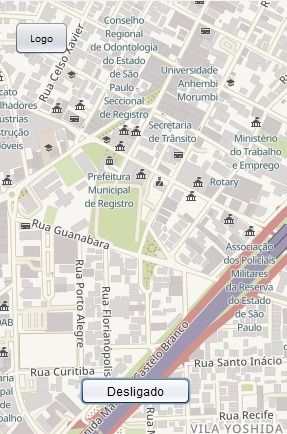
\includegraphics[width=0.5\linewidth]{Illustrations/Visi_Seco.jpg}
    \caption*{\textbf{Fonte: do próprio autor, 2024.}}
\end{figure}

\vspace{12pt}

A (Figura 4) Esta é a tela inicial do administrador, onde ele pode selecionar a doença que deseja visualizar no HeatMap, escolher a rota para enviar as equipes de dedetização e registrar uma localização de dengue.

\begin{figure}[H]
    \centering
    \caption{Tela 2}
    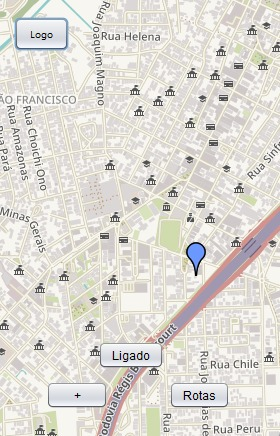
\includegraphics[width=0.5\linewidth]{Illustrations/Adm.jpg}
    \caption*{\textbf{Fonte: do próprio autor, 2024.}}
\end{figure}

\vspace{12pt}

 A (Figura 5) mostra a tela inicial do agente de saúde, o qual pode registar uma localização de foco de dengue e visualizar o HeatMap da doença.
 
\begin{figure}[H]
    \centering
    \caption{Tela 3}
    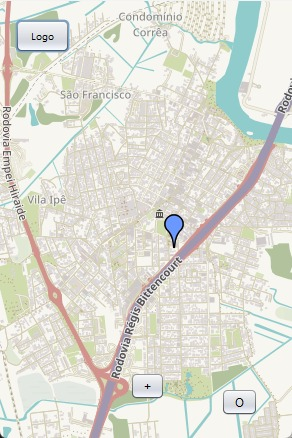
\includegraphics[width=0.5\linewidth]{Illustrations/Agente.jpg}
    \caption*{\textbf{Fonte: do próprio autor, 2024.}}
\end{figure}

\vspace{12pt}

A (Figura 6) indica a tela inicial do agente de dedetização, o qual terá acesso às possíveis rotas para o tratamento dos focos.

\begin{figure}[H]
    \centering
    \caption{Tela 4}
    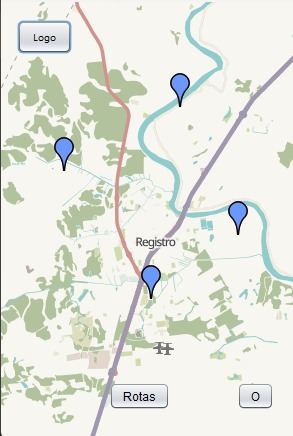
\includegraphics[width=0.5\linewidth]{Illustrations/Dedetizador.jpg}
    \caption*{\textbf{Fonte: do próprio autor, 2024.}}
\end{figure}

\vspace{12pt}

A (Figura 7) ilustra a tela inicial do visitante, o qual terá acesso apenas aos mapas de calor de dengue.

\begin{figure}[H]
    \centering
    \caption{Tela 5}
    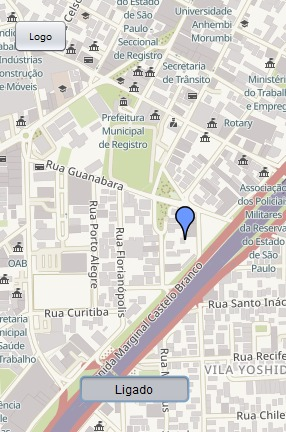
\includegraphics[width=0.5\linewidth]{Illustrations/Visitante.jpg}
    \caption*{\textbf{Fonte: do próprio autor, 2024.}}
\end{figure}

\vspace{12pt}

A (Figura 8) representa o mapa de calor da dengue. O mapa poderá ser visualizado pelo administrador, pelo agente de saúde e pelo visitante. 


\begin{figure}[H]
    \centering
    \caption{Tela 7}
    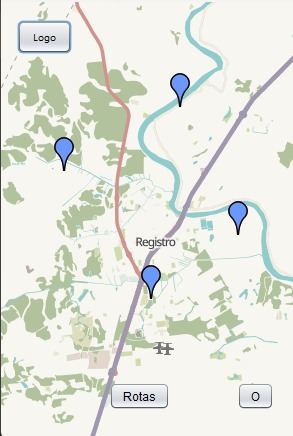
\includegraphics[width=0.5\linewidth]{Illustrations/mapa_calor.jpg}
    \caption*{\textbf{Fonte: do próprio autor, 2024.}}
\end{figure}

A (Figura 9) ilustra a tela de registro de localização de foco de dengue, atividade que poderá ser realizada pelo administrador ou agente de saúde.

\begin{figure}[H]
    \centering
    \caption{Tela 9}
    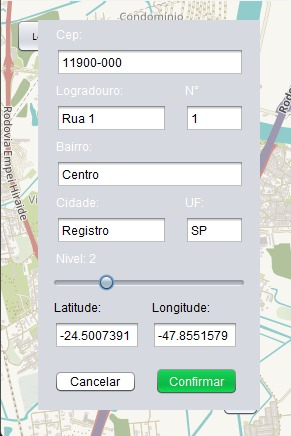
\includegraphics[width=0.5\linewidth]{Illustrations/Agt_cad.jpg}
    \caption*{\textbf{Fonte: do próprio autor, 2024.}}
\end{figure}


\vspace{12pt}

\textbf{Sistema em Node}\newline

O sistema foi inicialmente desenvolvido em Apex para facilitar a construção e visualização da aplicação web executável. A aplicação em Node.js visa proporcionar ao administrador uma visão geral da plataforma. Ela oferece ao gestor acesso total aos dados do sistema, permitindo a visualização dos agentes cadastrados, suas respectivas permissões e os celulares atribuídos a cada um. Além disso, o sistema registra os endereços onde foram identificados focos de dengue, acompanhados dos respectivos mapas de calor.

Essa abordagem visa fornecer ao administrador uma ferramenta eficiente para monitorar e gerenciar todos os aspectos relevantes da aplicação.

\vspace{12pt}

A (Figura 10) representam a aba de inserção do registro de um local com foco de dengue.

\begin{figure}[H]
    \centering
    \caption{Registro dengue}
    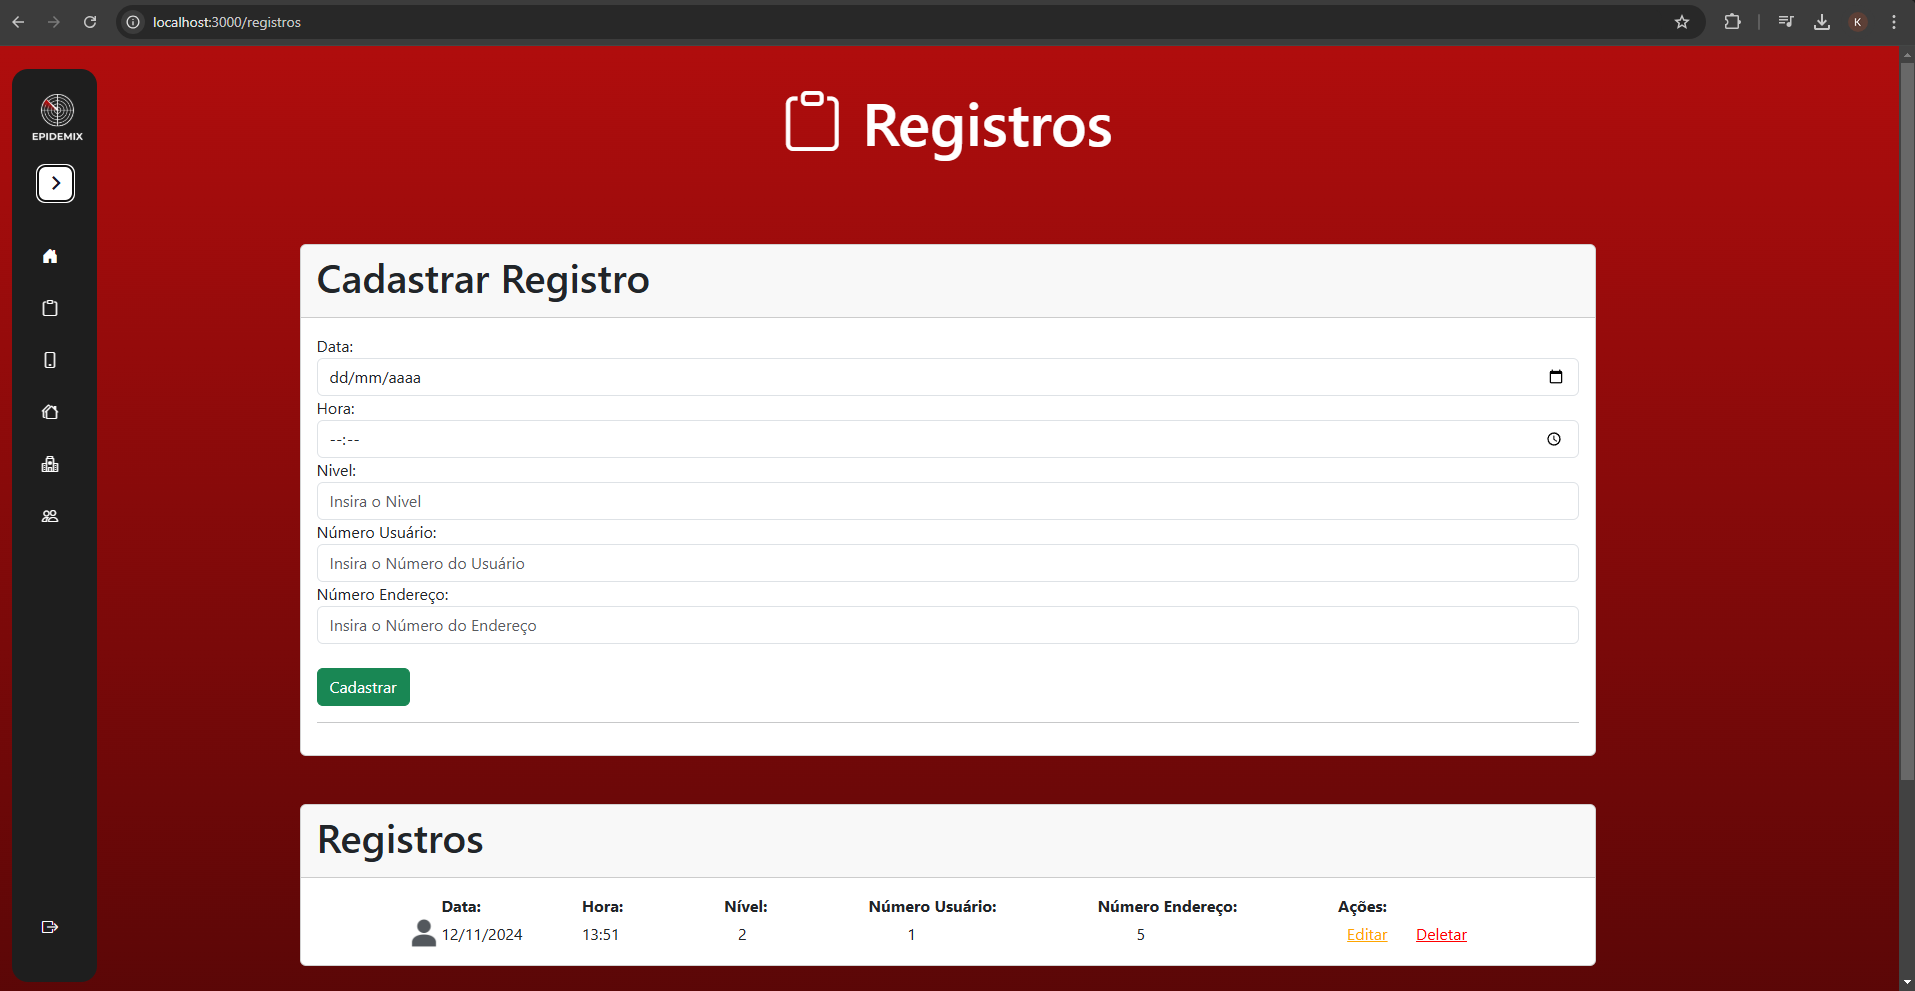
\includegraphics[width=1.0\linewidth]{Illustrations/Registro_Epidemix.png}
    \caption*{\textbf{Fonte: do próprio autor, 2024.}}
\end{figure}

\vspace{12pt}

A (Figura 11) mostra o mapa de calor de dengue com os pontos afetados por foco das doenças. 

\begin{figure}[H]
    \centering
    \caption{Mapa de calor dengue}
    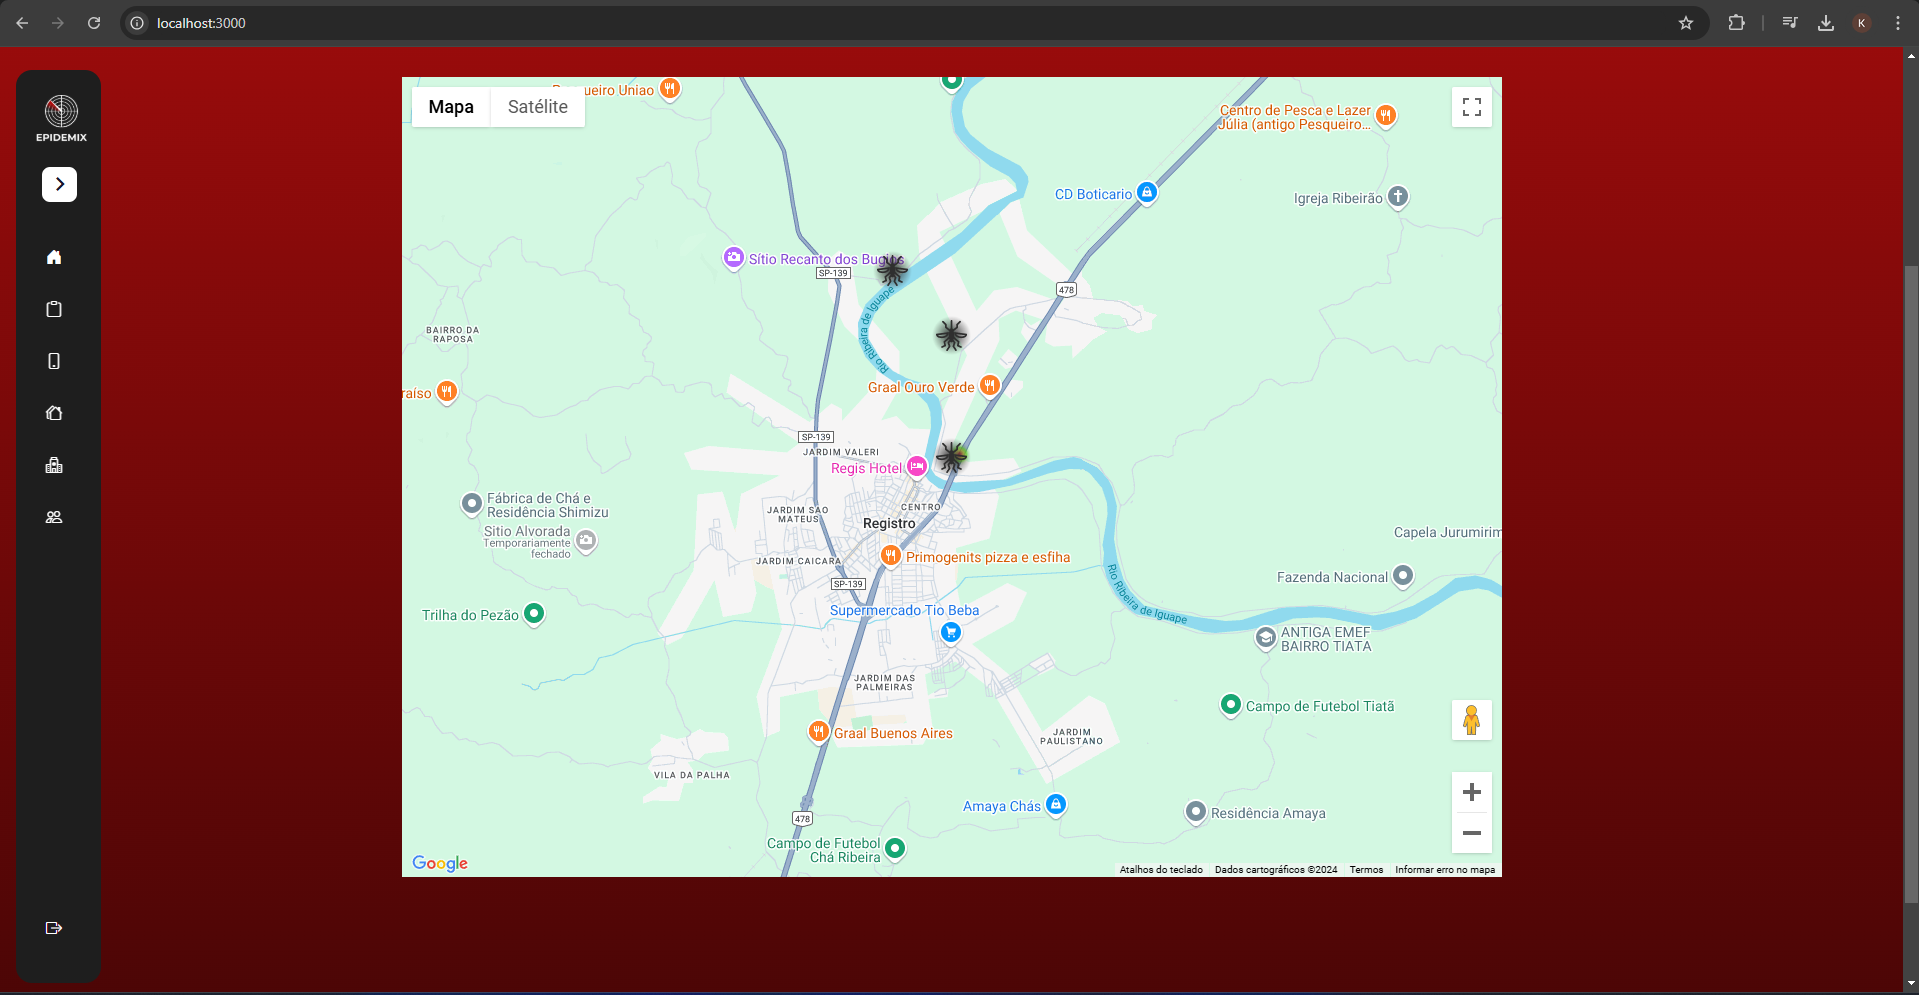
\includegraphics[width=1.0\linewidth]{Illustrations/Mapa de Calor.png}
    \caption*{\textbf{Fonte: do próprio autor, 2024.}}
\end{figure}

\vspace{12pt}


Na (Figura 12 e 13) é possível obervar os usuários e os celulares cadastrados. No caso, os usuários são os agentes e os celulares são os dispositivos utilizados para registrar uma localização.

\begin{figure}[H]
    \centering
    \caption{Usuários}
    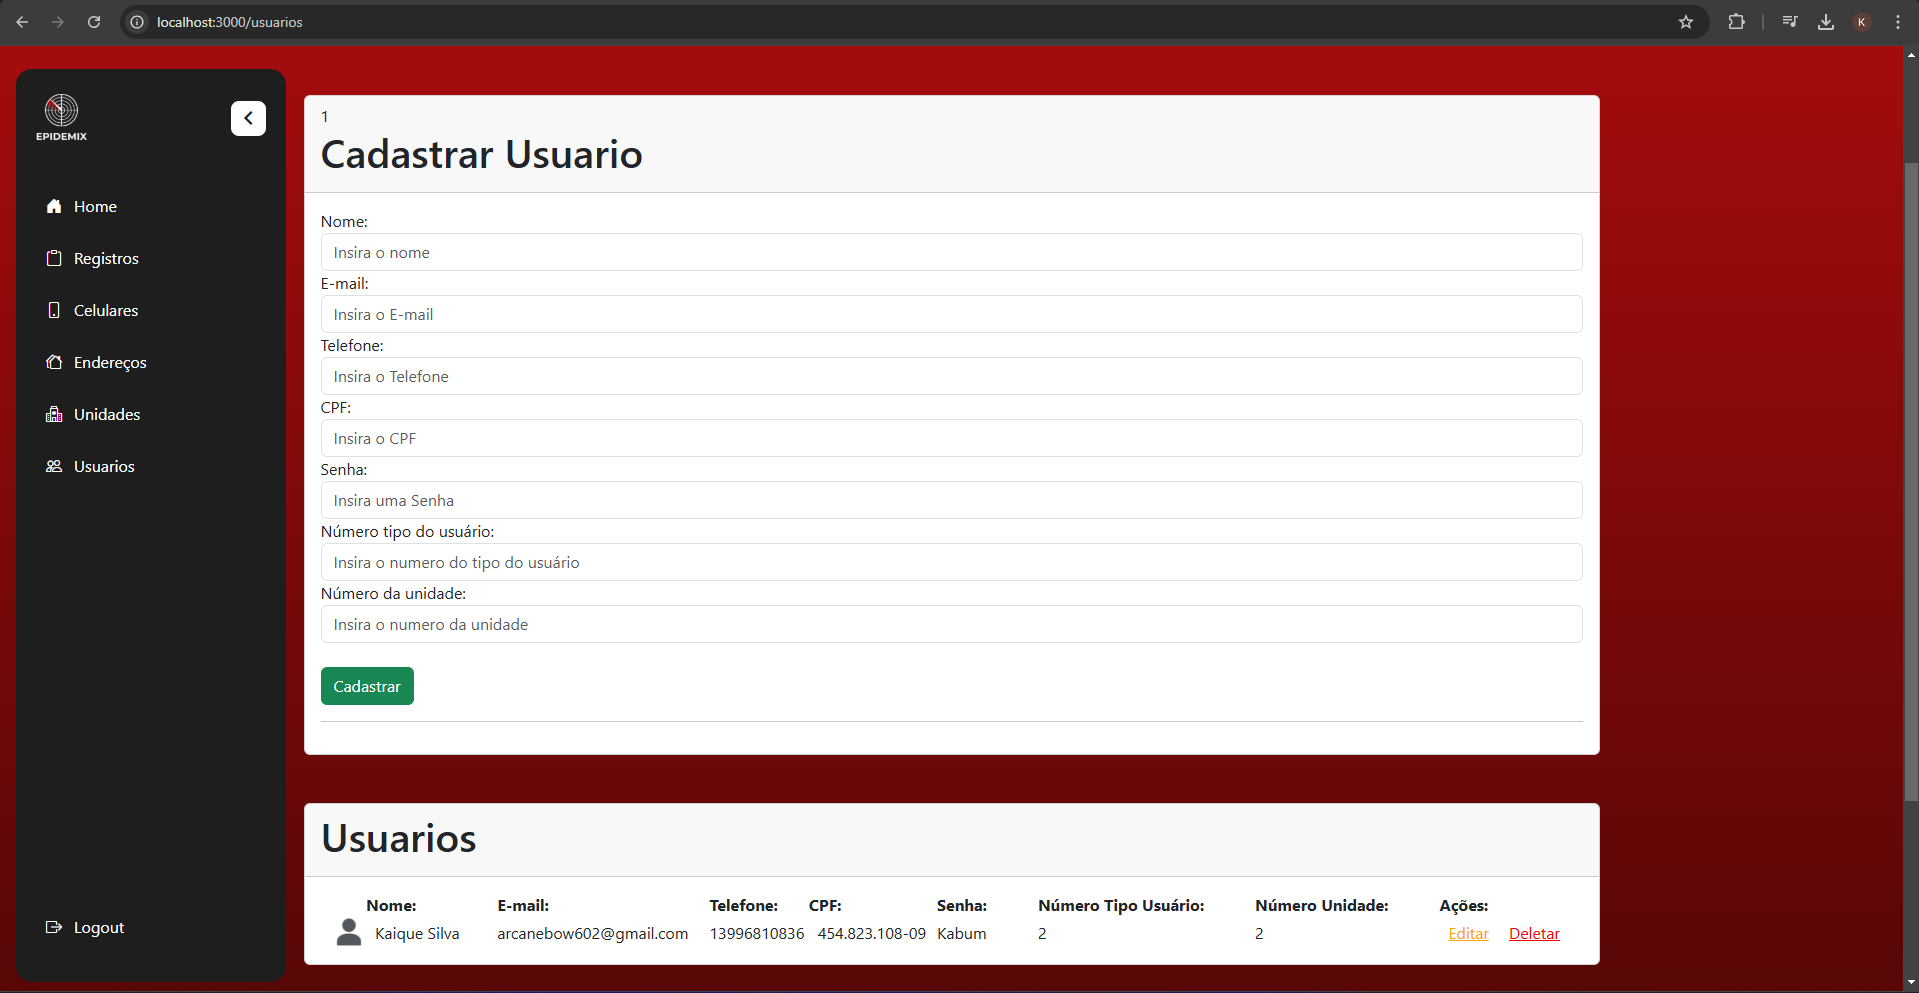
\includegraphics[width=1.0\linewidth]{Illustrations/Usuario.png}
    \caption*{\textbf{Fonte: do próprio autor, 2024.}}
\end{figure}

\vspace{12pt}

\begin{figure}[H]
    \centering
    \caption{Celulares}
    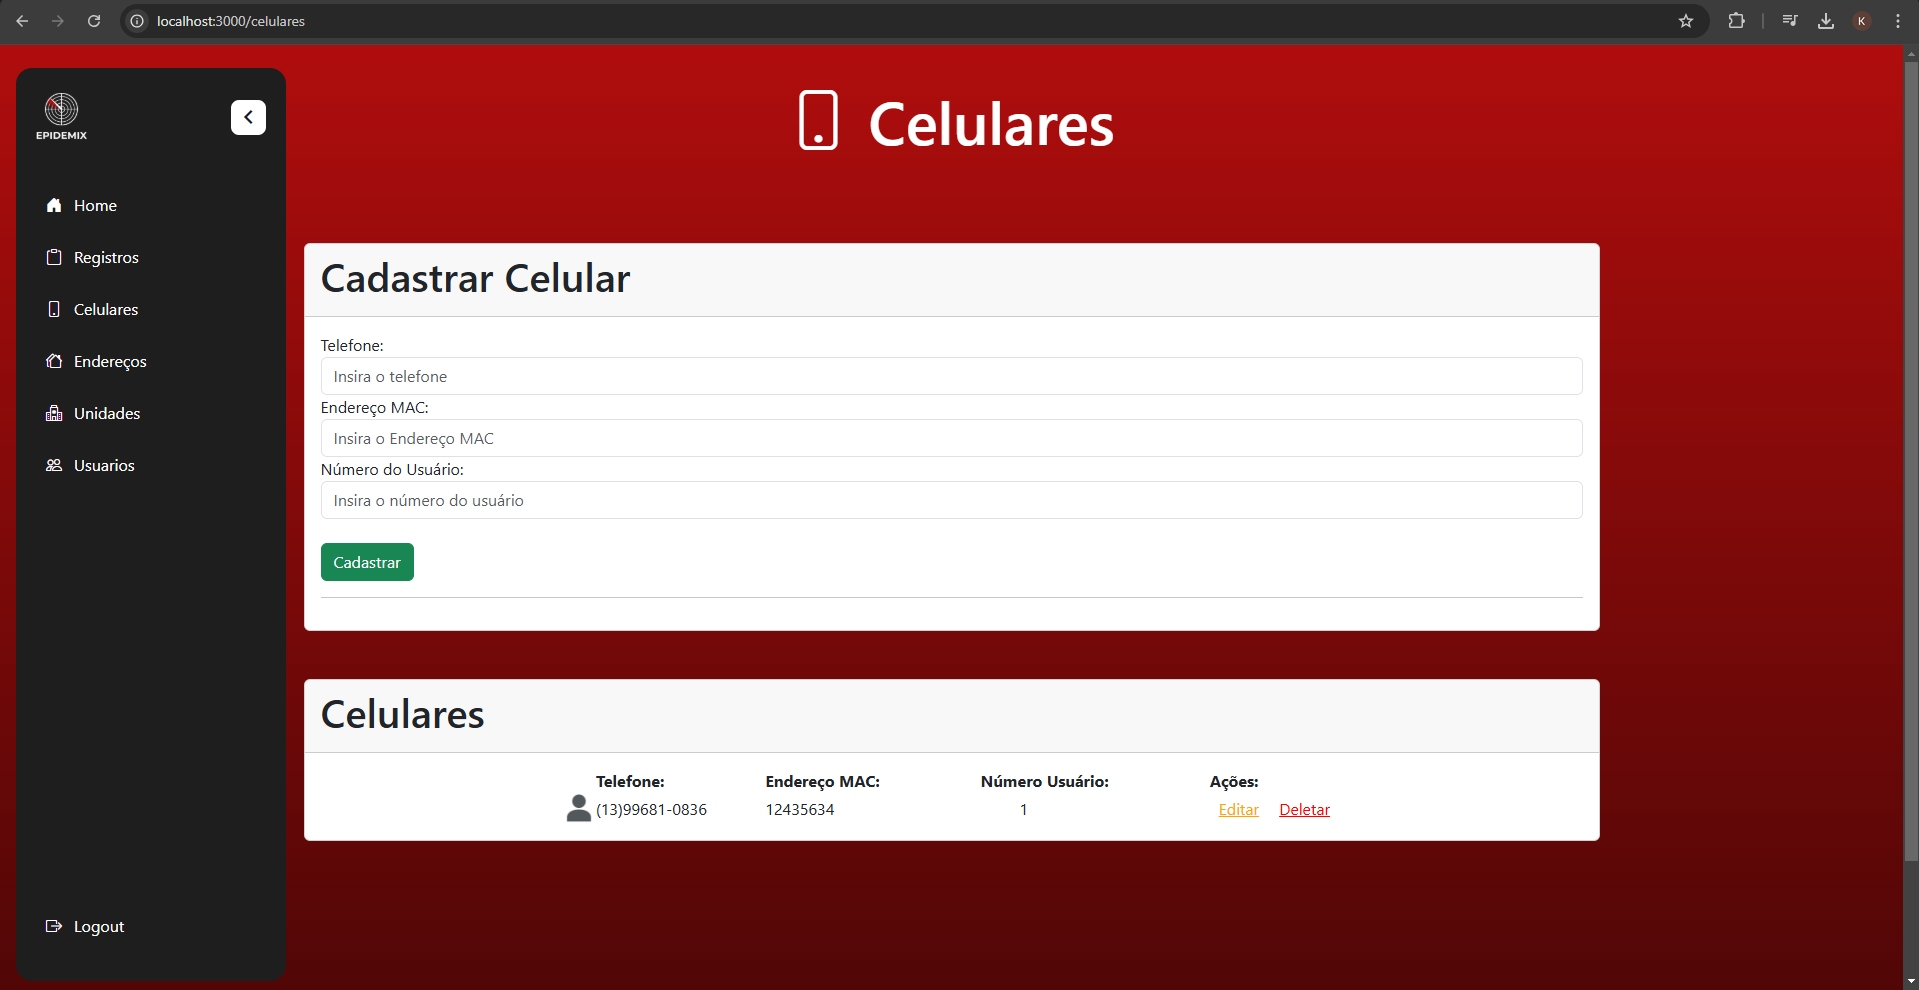
\includegraphics[width=1.0\linewidth]{Illustrations/celulares.png}
    \caption*{\textbf{Fonte: do próprio autor, 2024.}}
\end{figure}

\vspace{12pt}

A (Figura 14) mostra a aba Endereços, onde é possível observar as informações de uma localização afetada, como o endereço do local, o nível do risco e o agente responsável pelo registro. 

\begin{figure}[H]
    \centering
    \caption{Endereços}
    \includegraphics[width=1.0\linewidth]{Illustrations/Endereços.png}
    \caption*{\textbf{Fonte: do próprio autor, 2024.}}
\end{figure}

\vspace{12pt}

A (Figura 15) representa as unidades em que a equipe responde.

\begin{figure}[H]
    \centering
    \caption{Unidades}
    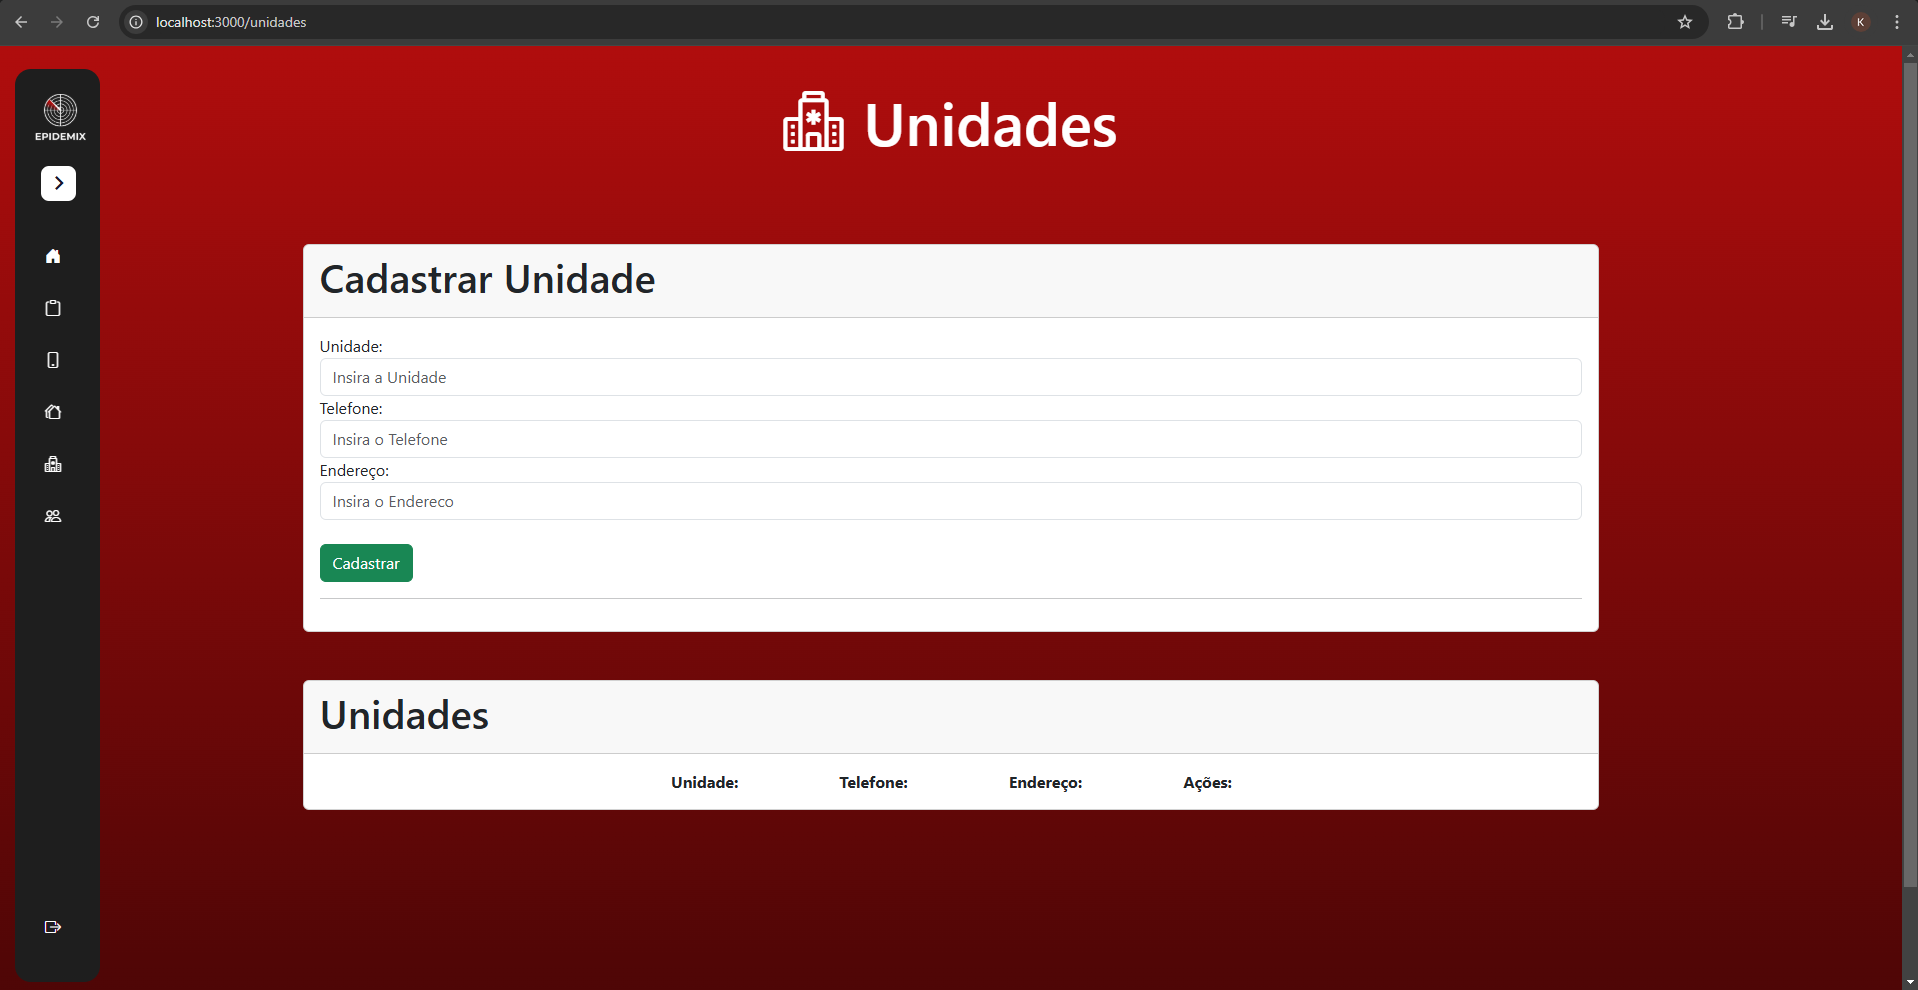
\includegraphics[width=1.0\linewidth]{Illustrations/Unidades.png}
    \caption*{\textbf{Fonte: do próprio autor, 2024.}}
\end{figure}

\vspace{12pt}


\textbf{Diagrama de caso de uso}\newline

A UML (Unified Modeling Language) do sistema serve para visualizar, especificar e documentar a estrutura e o comportamento externo do sistema de software. O diagrama fornece uma linguagem padronizada para comunicar as diferentes partes e aspectos que o sistema irá oferecer aos usuários, auxiliando no projeto, desenvolvimento e manutenção do software. 

Durante o desenvolvimento da UML, seis atores foram identificados. O super administrador, que faz referência ao dono do software, depende que o administrador envie dados pessoais e dados do departamento ao qual ele está cadastrado, para que o dono possa gerenciar os dados inseridos. Além disso, outras funcionalidades podem ser atribuídas a ele, como o gerenciamento do cadastro de um agente de saúde, o registro da localização afetada, a edição dos dados inseridos, e a criação e observação de relatórios. Outro ator reconhecido é o administrador/coordenador da equipe de saúde, responsável por administrar cadastros de agentes de saúde e por gerar e visualizar os relatórios. O registro da localização afetada e a edição de tais dados são outras funcionalidades que podem ser atribuídas a ele. O próximo ator é o agente de saúde, que envia dados pessoais para que o coordenador e o super administrador possam gerenciá-los. Sua principal função é registrar uma área com foco de dengue, mas também poderá visualizar os relatórios gerados pelos dados inseridos no sistema. O usuário civil foi identificado, este poderá apenas visualizar os mapas gerados com a intenção de reconhecer áreas afetadas e preservar sua saúde.

\begin{figure}[H]
    \centering
    \caption{Diagrama de caso de uso}
    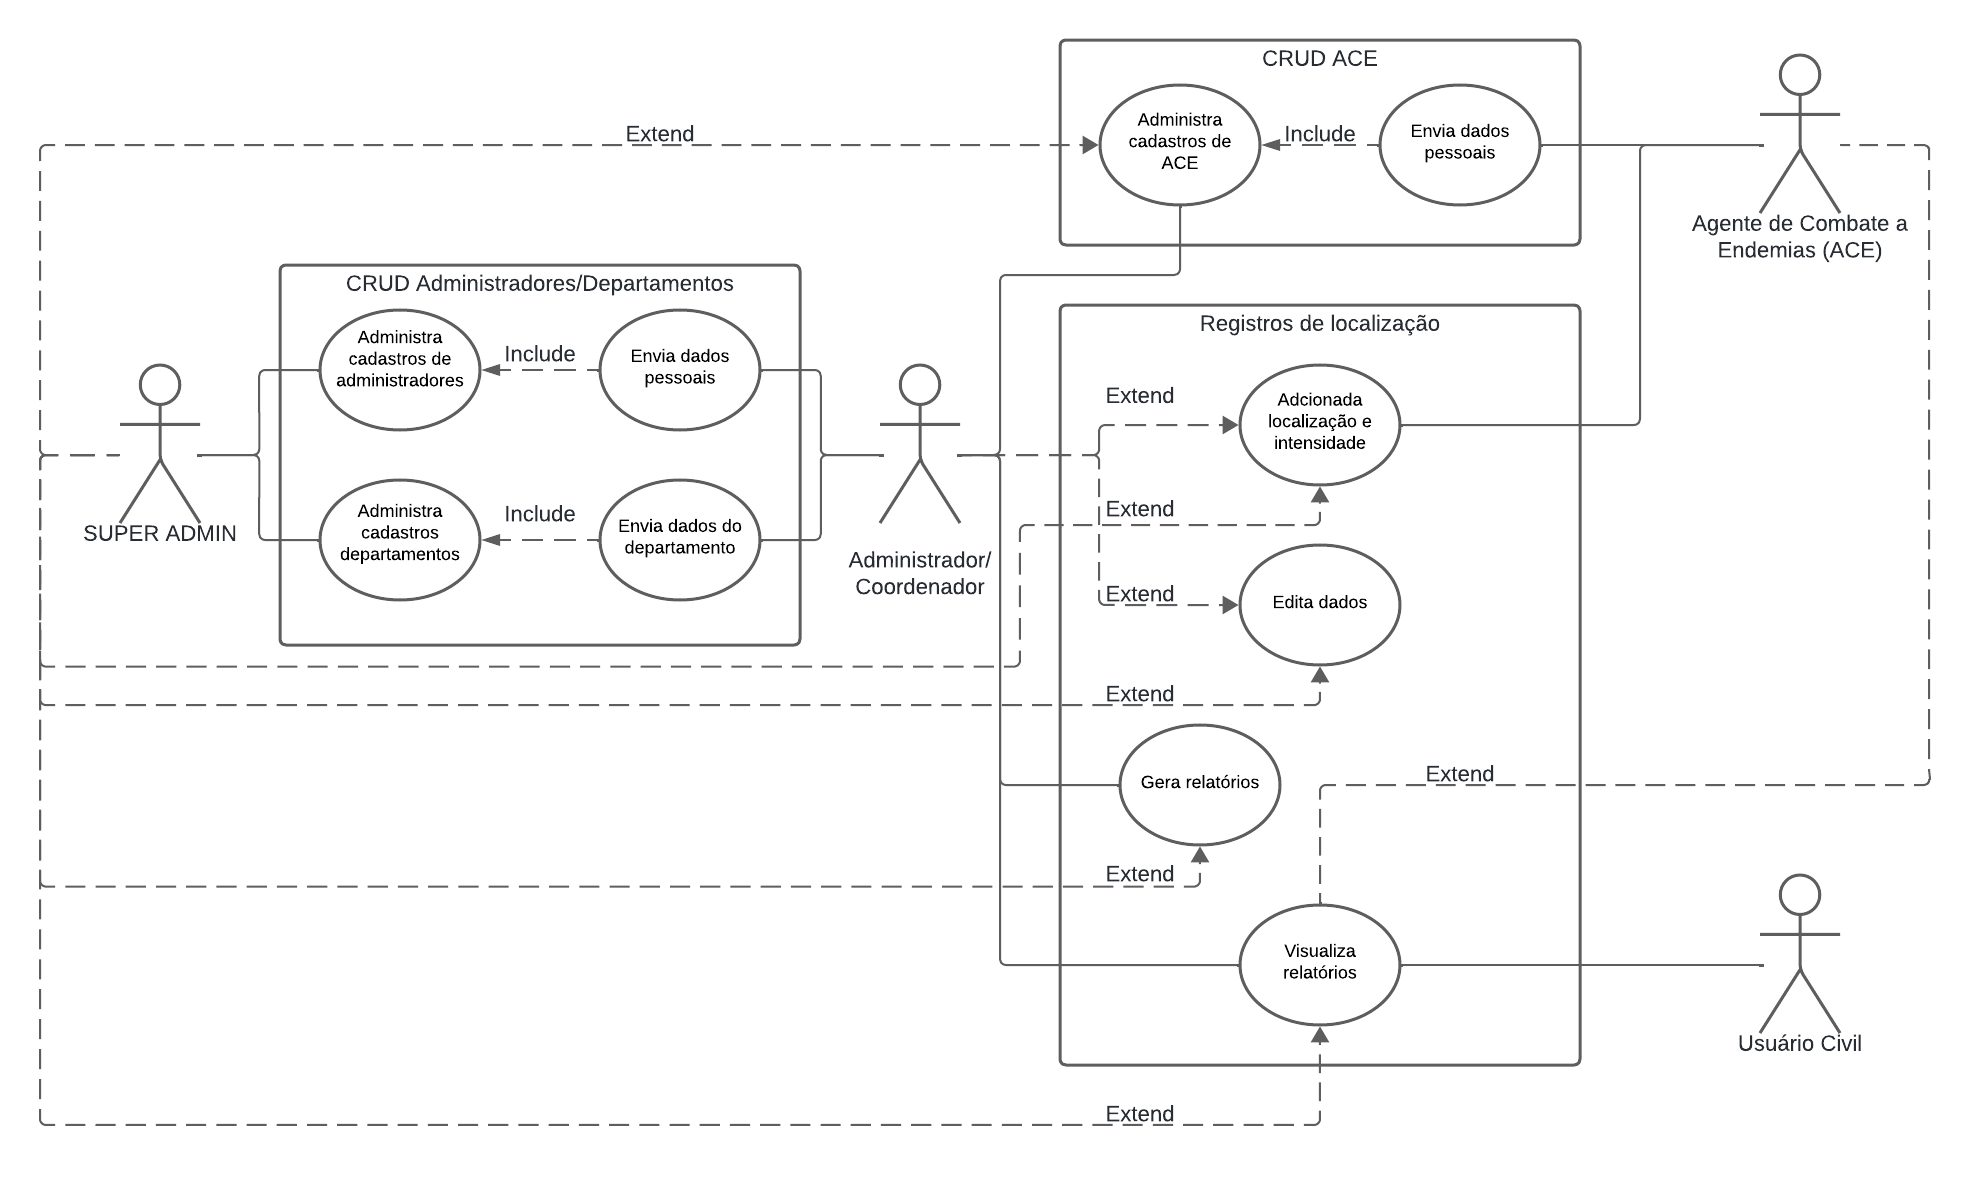
\includegraphics[width=1.0\linewidth]{Illustrations/uml1.png}
    \caption*{\textbf{Fonte: do próprio autor, 2024.}}
\end{figure}

\vspace{12pt}

Na continuação da UML, o gestor da equipe de saúde visualiza e encaminha as rotas geradas pela inteligência artificial para o agente dedetizador para que o tratamento do local possa ser realizado. Ainda cabe ao coordenador administrar os cadastros do agente dedetizador. Este, por sua vez, envia seus dados pessoais ao administrador, visualiza e finaliza as rotas de tratamento. A finalização da rota também pode ser realizada pelo coordenador. 

\begin{figure}[H]
    \centering
    \caption{Diagrama de caso de uso}
    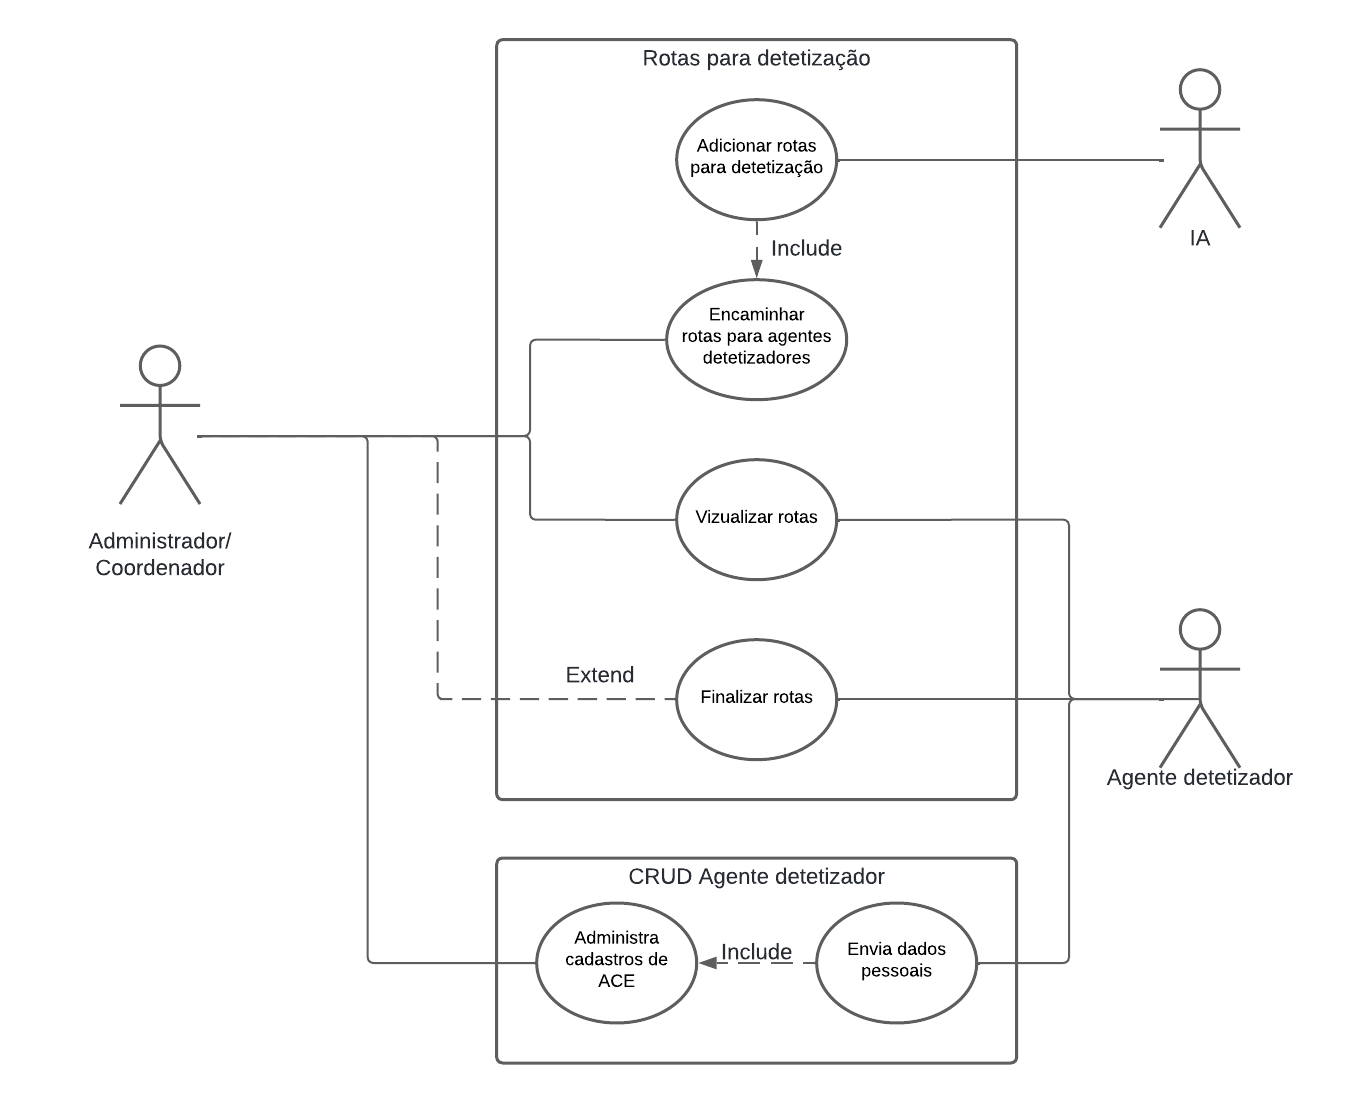
\includegraphics[width=1.0\linewidth]{Illustrations/uml2.png}
    \caption*{\textbf{Fonte: do próprio autor, 2024.}}
\end{figure}

\vspace{12pt}

É importante observar que foram criados dois diagramas separados, pois a plataforma em que foram desenvolvidos possui limite de elementos a serem utilizados. 

\vspace{12pt}

\textbf{Diagrama de redes}\newline

O diagrama de redes do sistema serve como uma representação visual da infraestrutura de rede, destacando dispositivos, conexões e a topologia geral. Sendo assim, facilita a compreensão da arquitetura da rede, ajudando na identificação de componentes individuais e suas interconexões. Em suma, o diagrama de redes é essencial para gerenciamento eficaz da infraestrutura de rede da aplicação. 

O diagrama de redes foi estruturado da seguinte forma: o agente de saúde acessa o aplicativo através do celular por meio da rede, e, consequentemente, qualquer alteração feita por ele será armazenada na nuvem. Por outro lado, o administrador terá acesso total à infraestrutura de rede, ou seja, será capaz de visualizar as alterações feitas pelo agente e salvas na nuvem, refletidas no aplicativo EPIDEMIX armazenado no servidor.

\begin{figure}[H]
    \centering
    \caption{Diagrama de redes}
    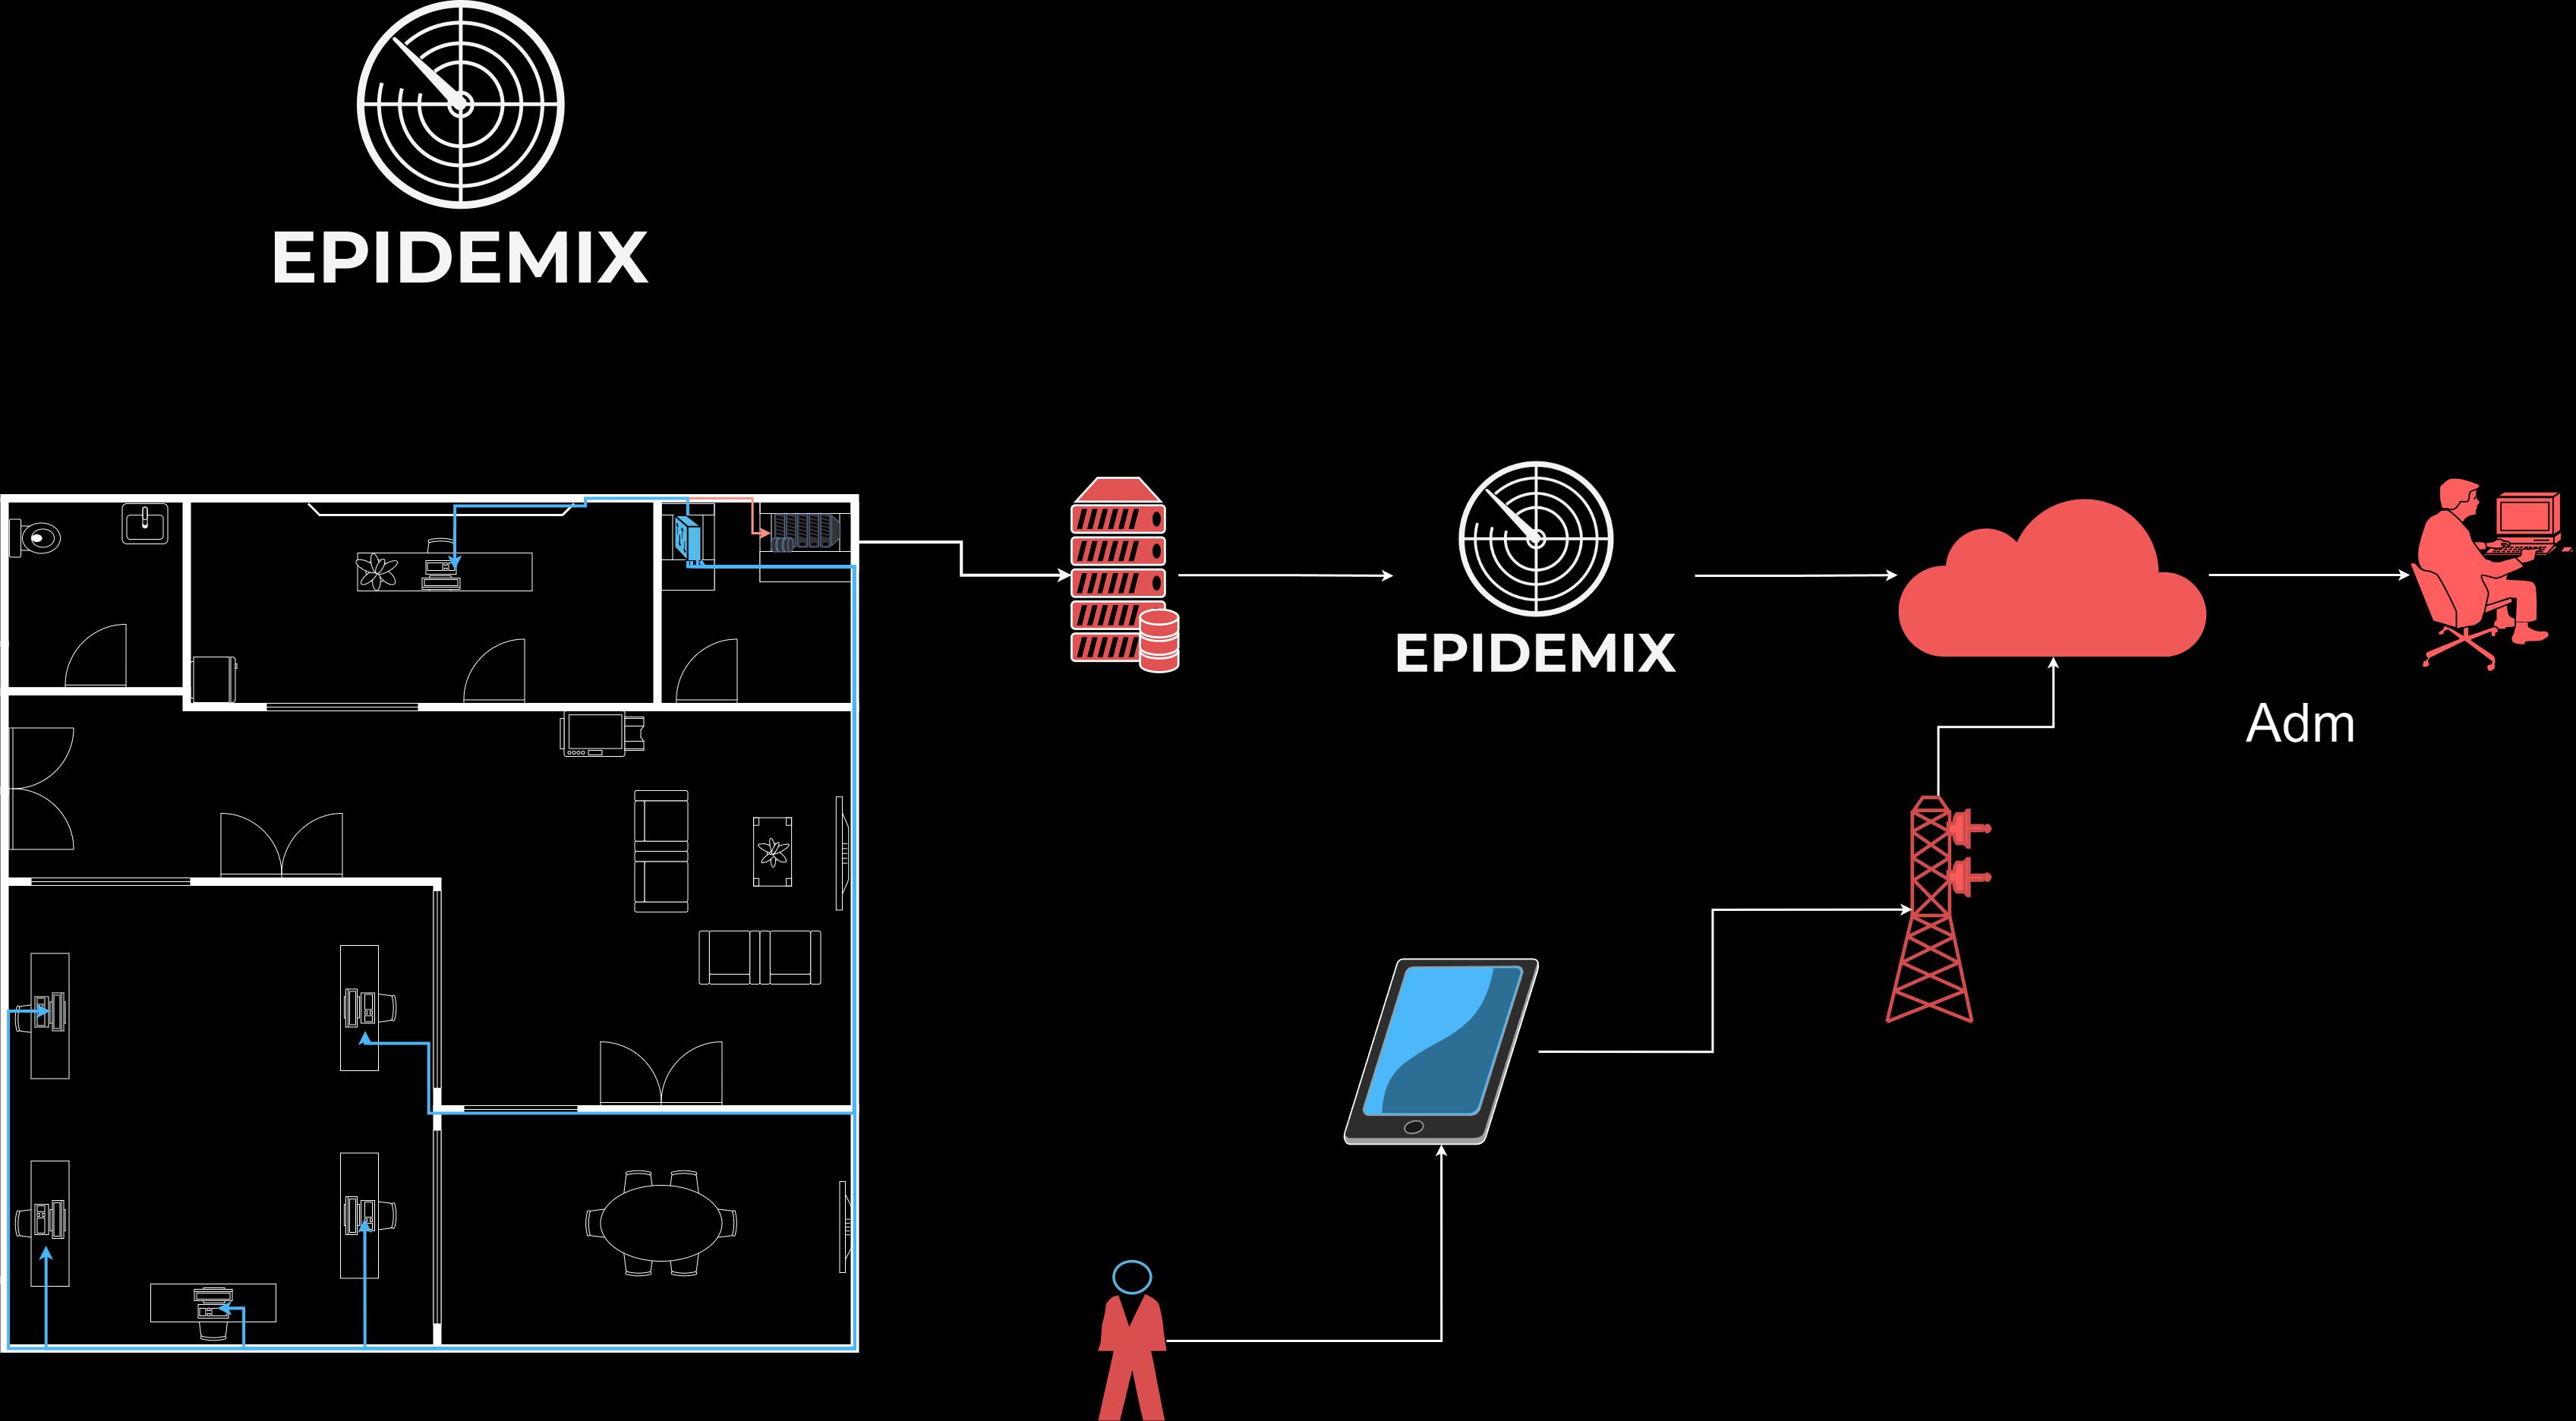
\includegraphics[width=1.0\linewidth]{Illustrations/redes.png}
    \caption*{\textbf{Fonte: do próprio autor, 2024.}}
\end{figure}

\vspace{12pt}

\textbf{Modelagem de banco de dados}\newline

O modelo de banco de dados conceitual delineia os requisitos de dados de forma abstrata, facilitando a compreensão dos relacionamentos entre entidades no sistema. Já o modelo lógico traduz esses conceitos em estruturas de dados concretas, permitindo sua implementação técnica. Juntos, esses modelos fornecem uma base sólida para o design e desenvolvimento do banco de dados da aplicação, garantindo consistência e eficiência. 

Ao acessar o aplicativo, o usuário irá realizar o login na seção em que ele se enquadra, fazendo referência à entidade "Tipos-usuário". O tipo de usuário varia entre administrador da equipe, agente de saúde, agente de dedetização e visitante, os quais possuem suas respectivas permissões. O Usuário já estará cadastrado na entidade "Users" com as seguintes informações: nome completo, e-mail, telefone, CPF e senha. Cada profissional terá um celular vinculado a ele de acordo com o endereço MAC do aparelho, e também estará relacionado à unidade a qual ele responde, o hospital será identificado pelo nome e telefone de contato. Após o usuário realizar o login com seu e-mail e senha, poderá fazer o registro da localização de dengue. No registro da doença é necessário inserir o endereço, a data, a hora e o nível do foco identificado.

\begin{figure}[H]
    \centering
    \caption{Banco de dados modelo conceitual}
    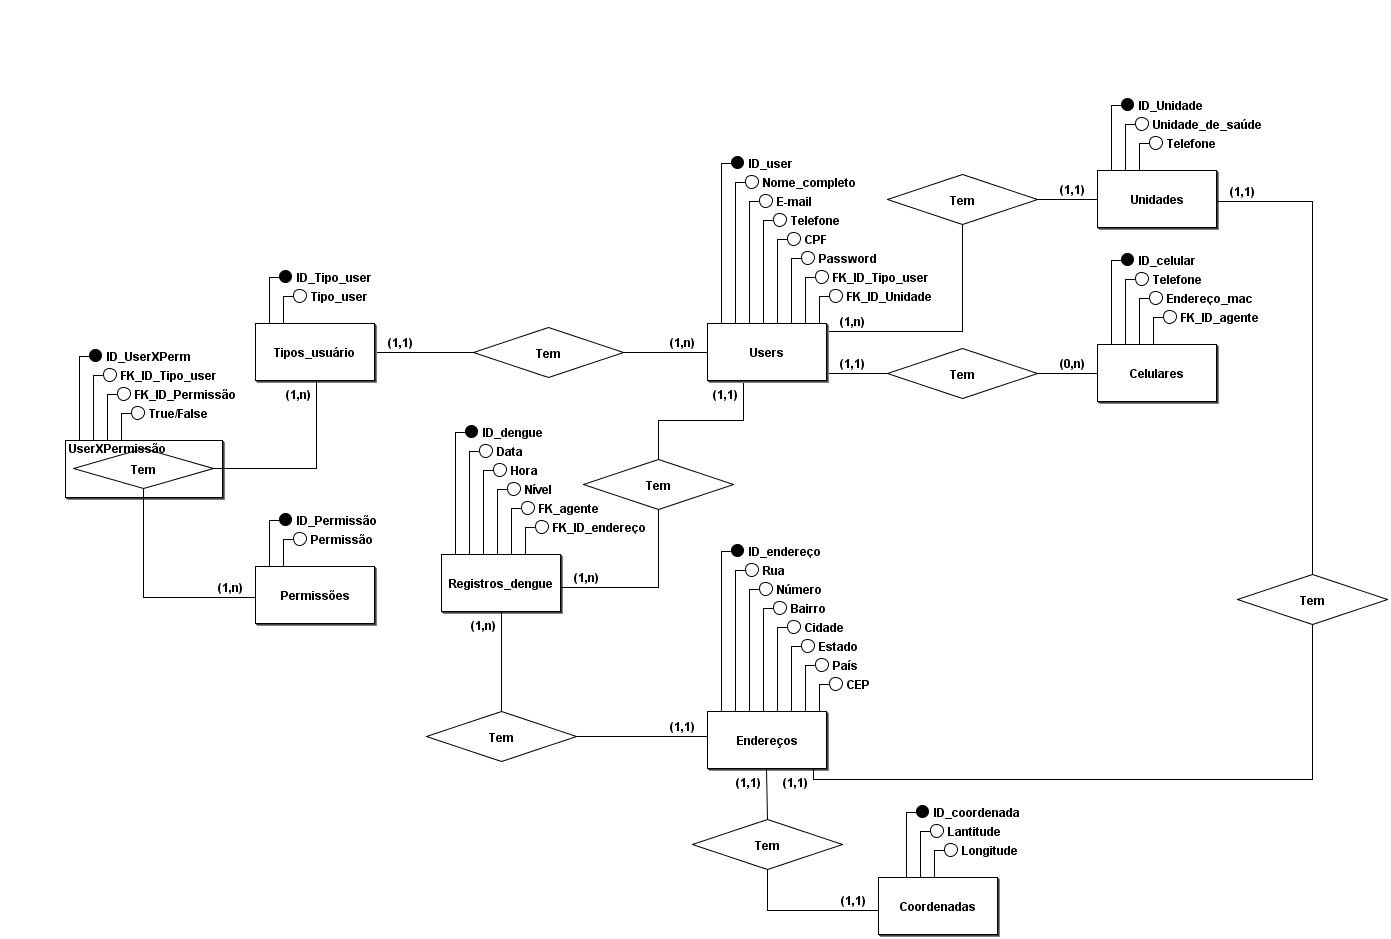
\includegraphics[width=1.0\linewidth]{Illustrations/Modelo_Conceitual Epidemix.png}
    \caption*{\textbf{Fonte: do próprio autor, 2024.}}
\end{figure}

\begin{figure}[H]
    \centering
    \caption{Banco de dados modelo lógico}
    \includegraphics[width=1.0\linewidth]{Illustrations/Modelo_Lógico_Epidemix.png}
    \caption*{\textbf{Fonte: do próprio autor, 2024.}}
\end{figure}

\vspace{12pt}

\textbf{Modelo de negócio Lean Canvas}\newline

O modelo de negócios Lean Canvas proporciona a clara compreensão de cada aspecto do modelo de negócio e dos elementos-chave do sistema EPIDEMIX. O objetivo é fornecer suporte de mapeamento com classificação de áreas de foco de dengue aos agentes de saúde de forma prática e simples, tanto no momento da administração dos dados quanto no momento de visualizá-los, por meio de dados em tempo real. Pretende-se utilizar o auxílio de inteligência artificial para gerar rotas entre os locais com focos da doença de forma eficiente, amenizando tempo e recursos. Ademais, buscamos fornecer outras informações importantes ao cliente por meio do WhatsApp, telefone ou reuniões. Canais de comunicação como mídias sociais e website foram estabelecidos. A atividade principal se baseia em um agente de saúde fazer o registro de uma localização com foco do Aedes aegypti em um mapa disponível na aplicação. Para isso, um dos recursos necessários é um dispositivo como celular, tablet ou computador com acesso à internet e GPS. O principal parceiro do sistema será o departamento de saúde pública. As despesas envolvem custos fixos, como salário de funcionários, hospedagem de website e hospedagem em servidor, internet (local e dados móveis), energia e locação de espaço, e também custos variáveis, como aquisição de hardwares e impostos. Em contrapartida, as fontes de renda variam entre o aluguel do software, aluguel de dispositivos para o registro dos dados e uma equipe para coleta e registro de dados, junto a um administrador/coordenador de equipes.

\begin{figure}[H]
    \centering
    \caption{Modelo de negócio Lean Canvas}
    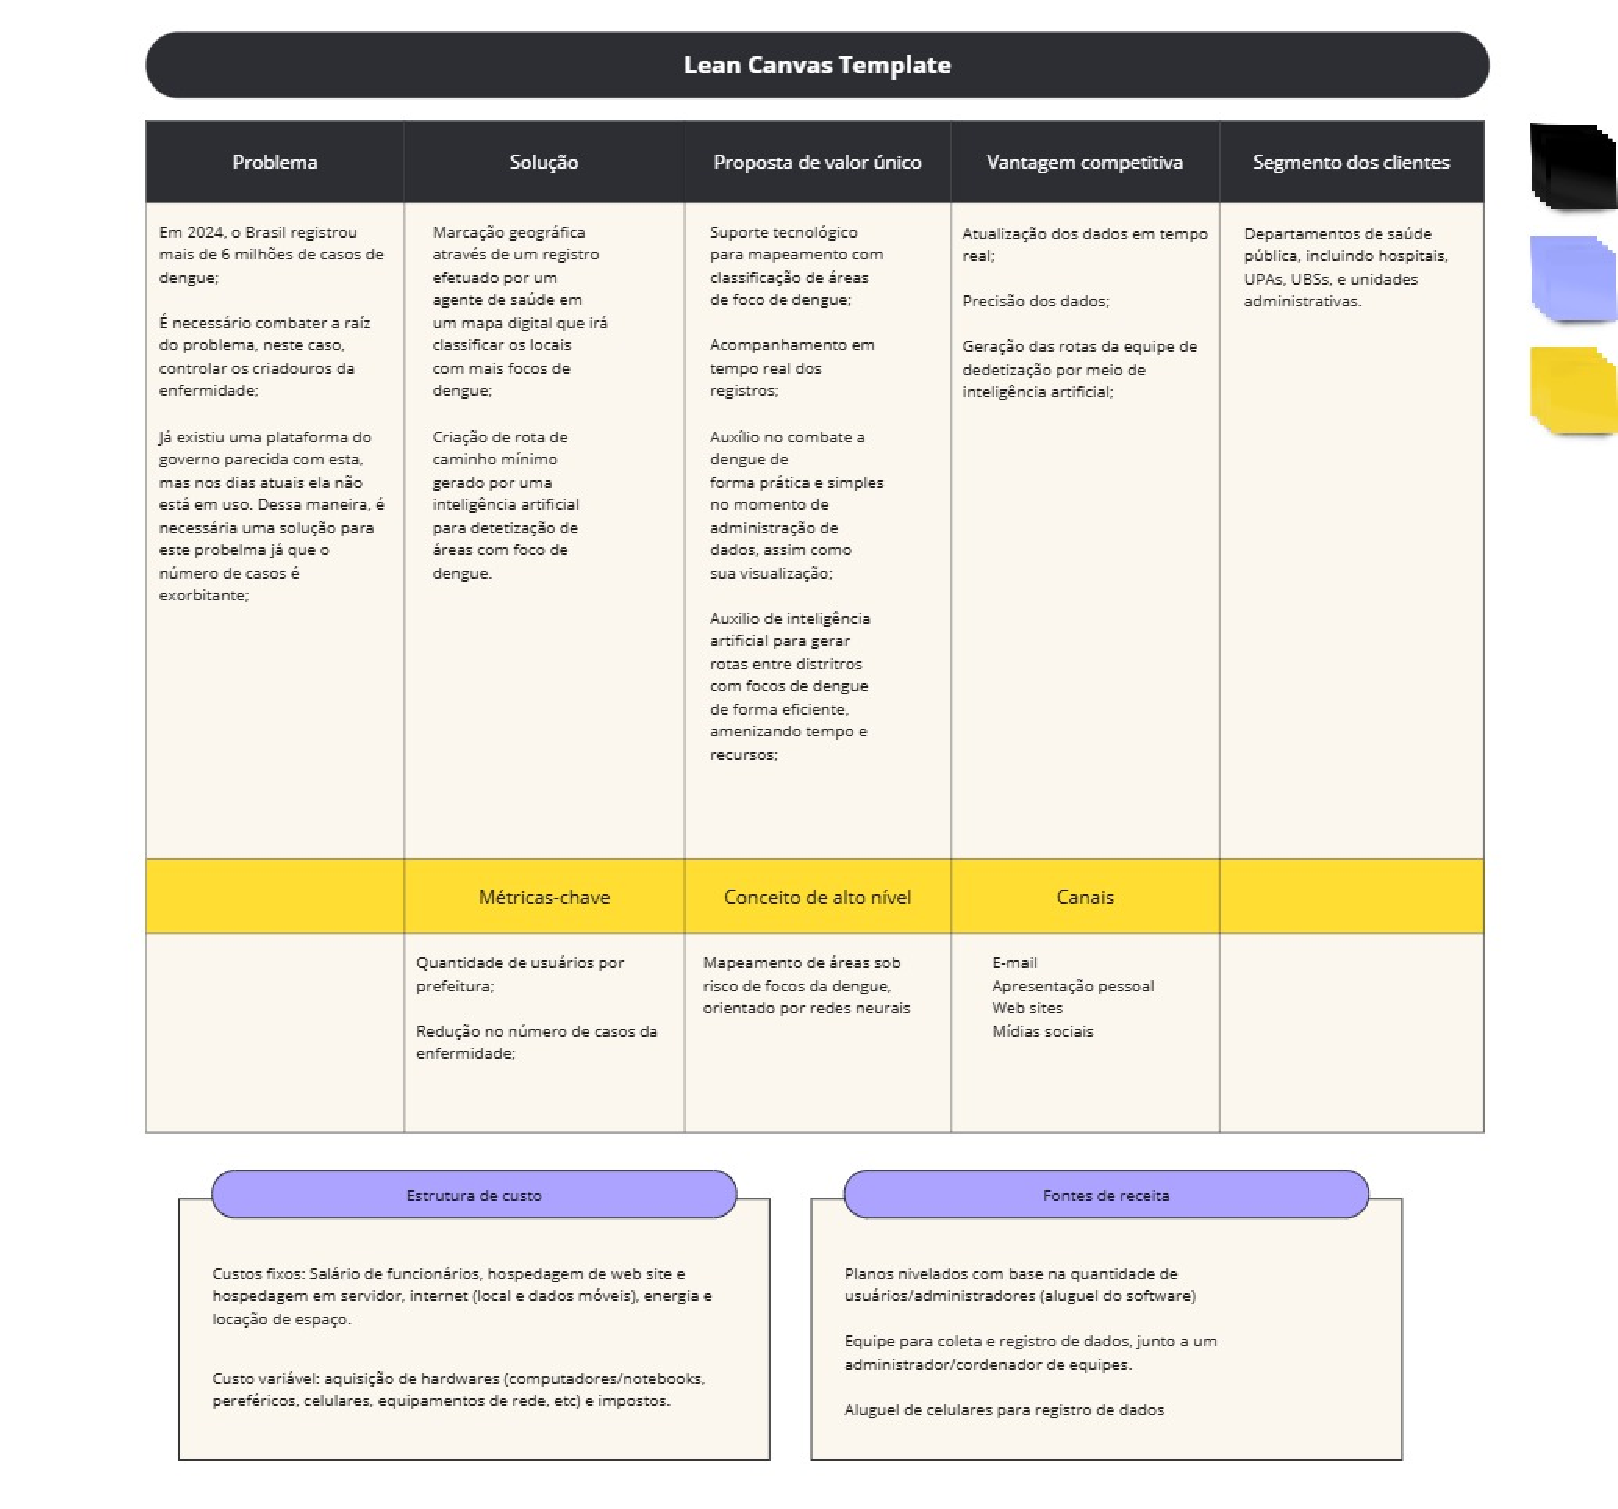
\includegraphics[width=1.0\linewidth]{Illustrations/Lean Canvas_Epidemix.pdf}
    \caption*{\textbf{Fonte: do próprio autor, 2024.}}
\end{figure}

\vspace{12pt}
